\section{Neural Network Architecture Exploration}
\label{sec:exploration}

We evaluated a number of neural network architectures with varying levels of structure and complexity before arriving at {\tool}'s network architecture (Section~\ref{sec:model}).

\begin{figure}
    \centering
    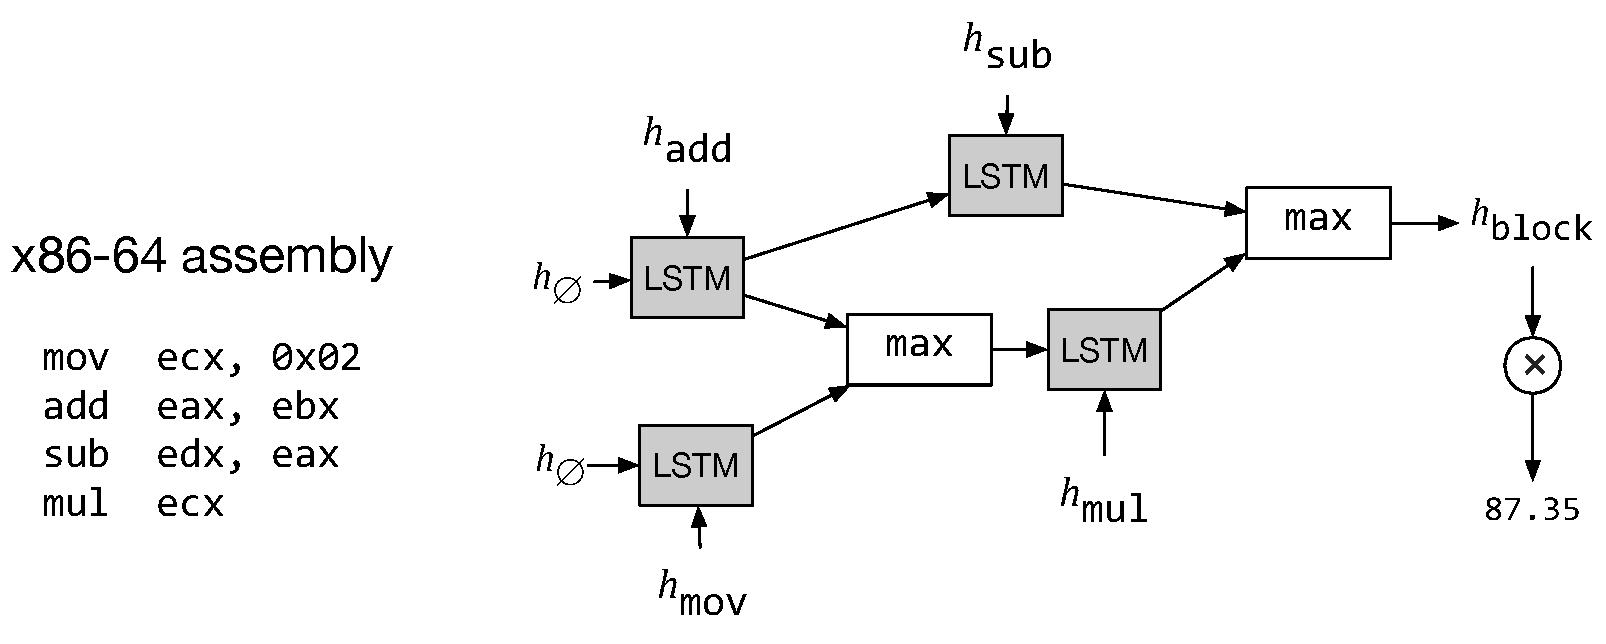
\includegraphics[width=\linewidth]{figures/diag_3architectures.pdf}
    \vspace{-20pt}
    \caption{The DAG-RNN Architecture}
    \label{fig:diff-networks}
\end{figure}

Figure~\ref{fig:diff-networks} shows a DAG-RNN~\cite{dag-rnn1, dag-rnn2}.
Instructions are embedded identically as to in \tool{} (i.e. the token layer and instruction layer remain the same).
However rather than running an RNN sequentially over the instructions in the prediction layer, the DAG-RNN constructs a dependence graph of the instructions in the basic block, with a directed edge between a pair of instructions if the second instruction depends on an output of the first instruction.
Because an instruction can depend on multiple previous instructions, we apply an element-wise max to reduce the states feeding in to a given instruction.
Then, the DAG-RNN applies an LSTM cell, using the generated instruction embedding as the input, and the result of the element-wise max as the input state.
To generate the final prediction, we take an element-wise max of the output states of all leaf instructions (all instructions with no dependents), and pass the result through a linear layer.

The DAG-RNN is inspired by the theoretical behavior of a perfect out-of-order processor: the throughput of a basic block running on a perfect out-of-order processor is equivalent to the throughput of the longest path that must be serially executed in that basic block.
Using a DAG-RNN implicitly encodes this prior, by only allowing information to propagate through the paths that must be serially executed in the block.

We also tested a simple token-level RNN with LSTM cells, which has a similar base architecture as \tool{}, but without the topmost prediction layer.
Instead, this model sequentially consumes all tokens in a basic block making no explicit distinction between instructions, giving a baseline measure for the efficacy of \tool{}'s hierarchical model.
The full architecture diagram for the token-level RNN is shown in Appendix~\ref{app:token-rnn-architecture}.

\begin{figure}[h!]
  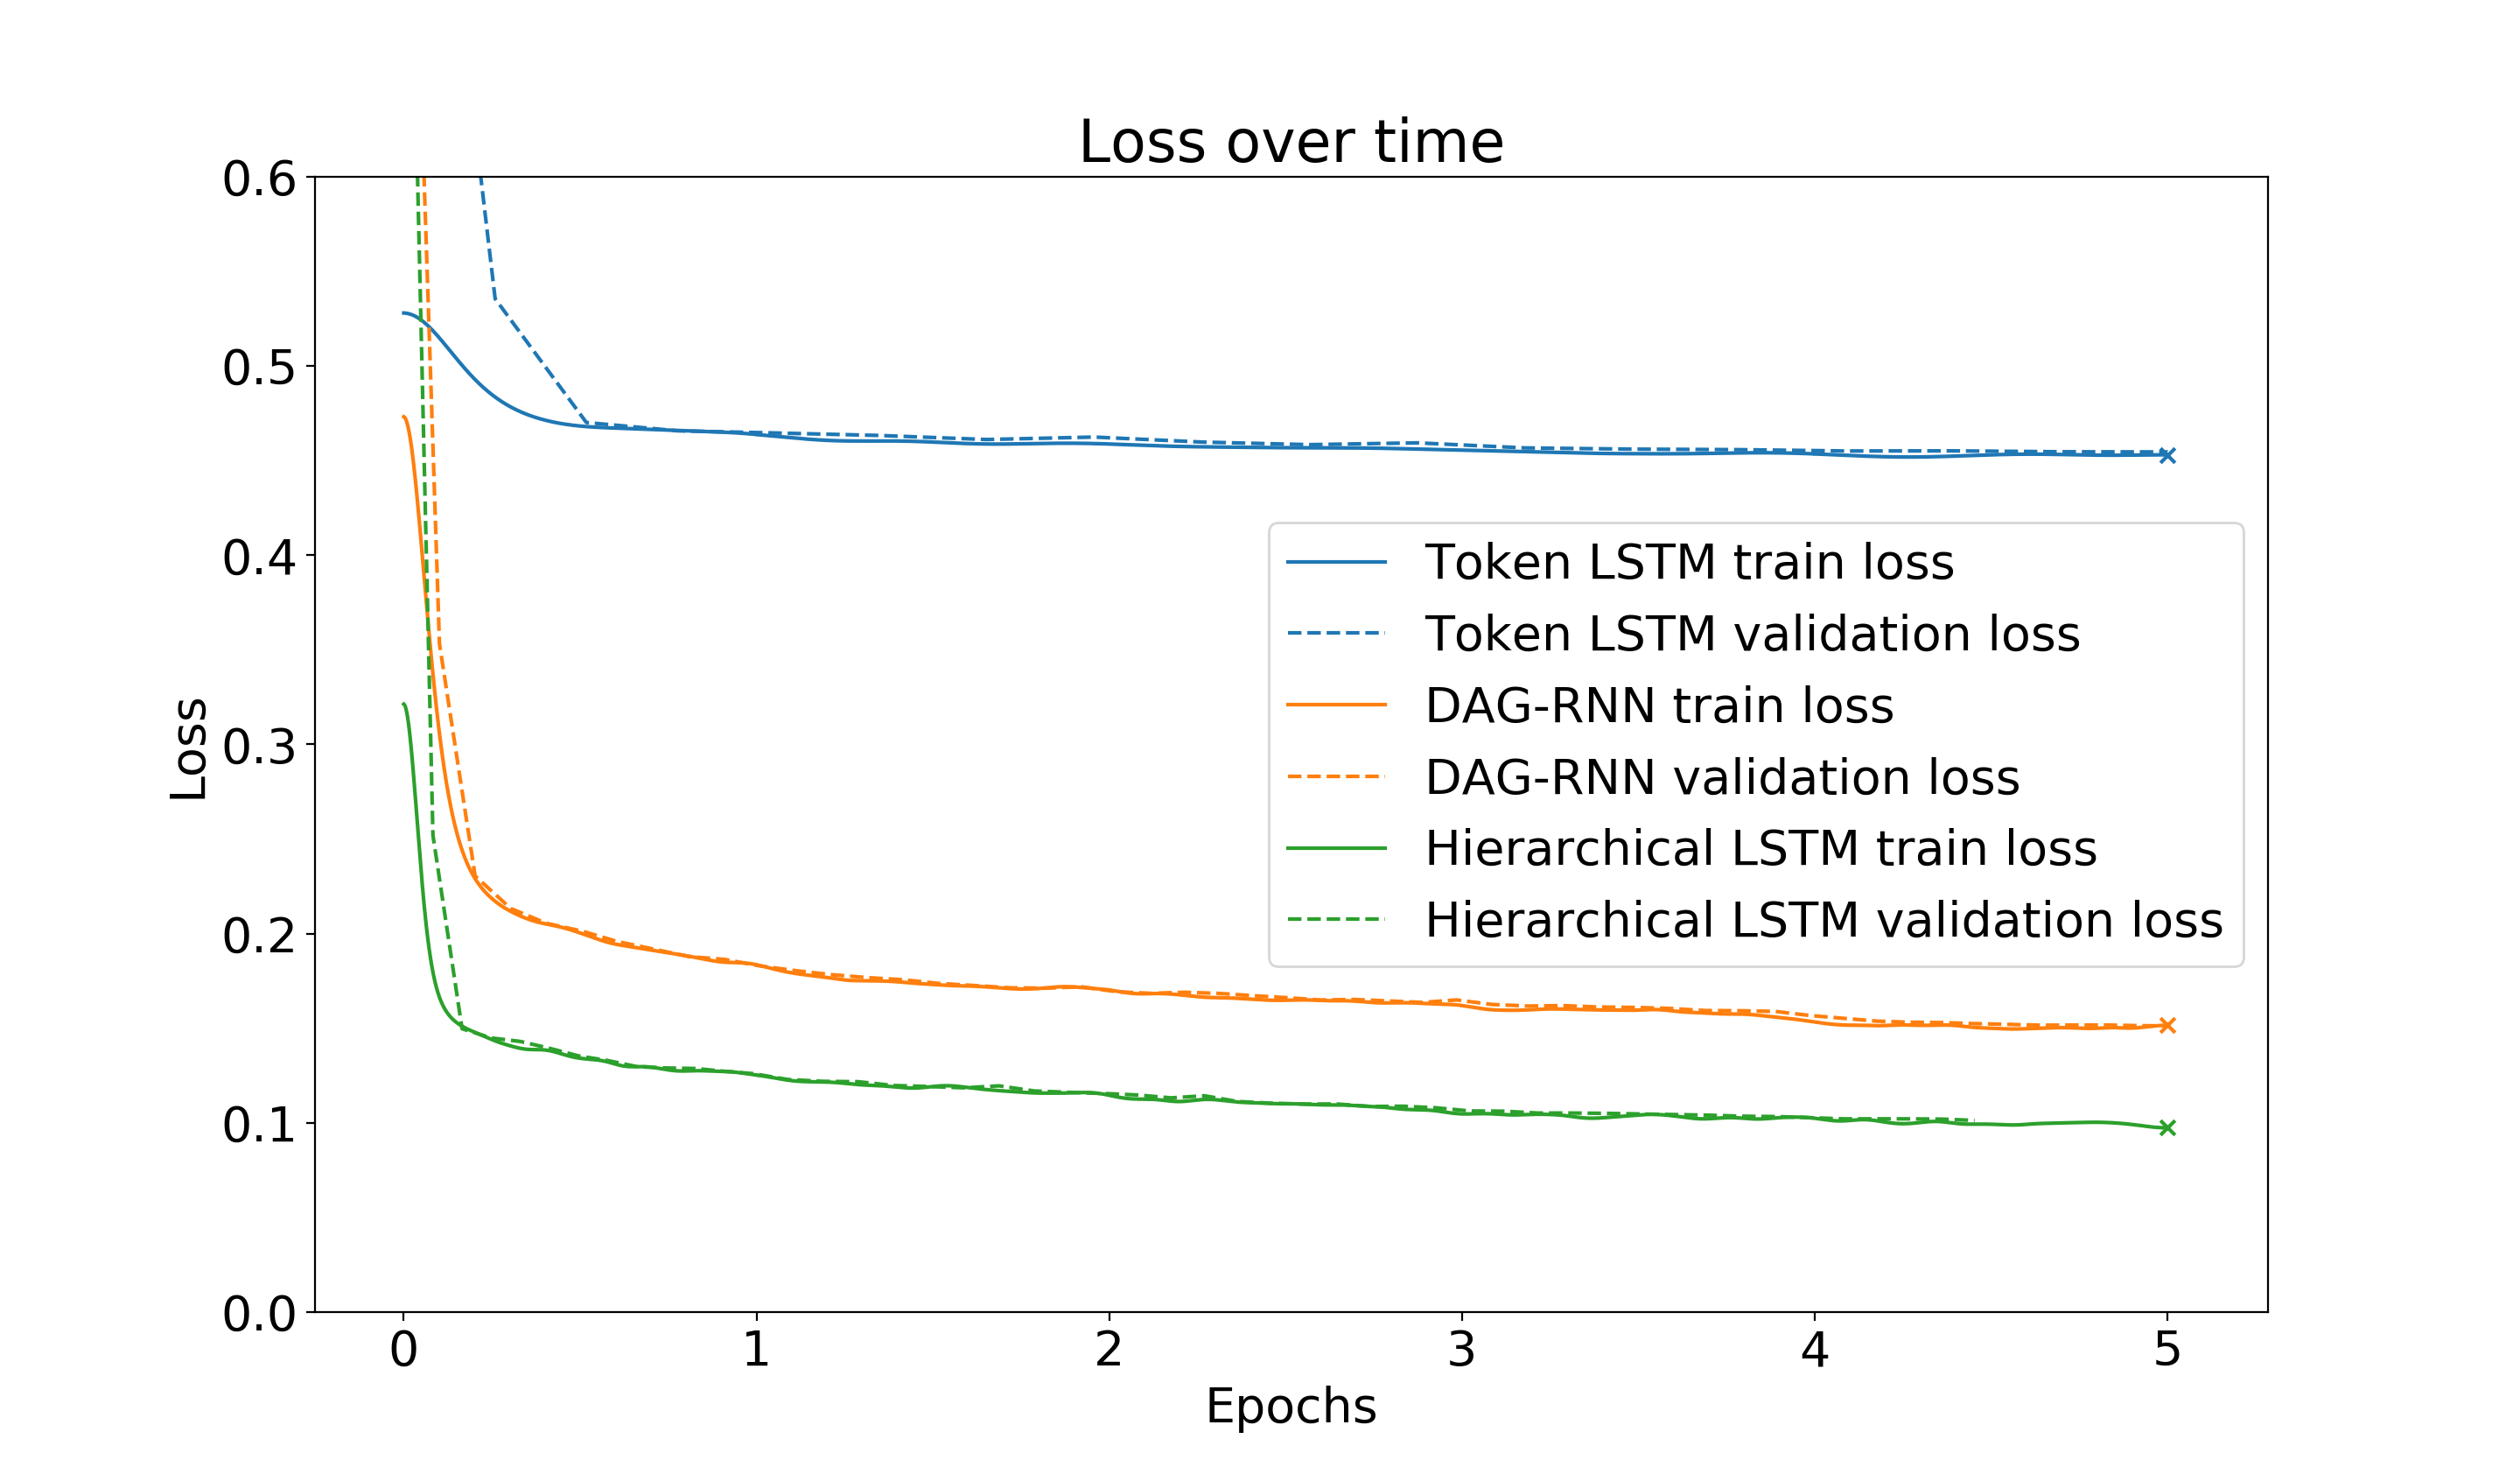
\includegraphics[width=\linewidth]{figures/architecture_search.png}
  \vspace{-20pt}
  \caption{Learning curves for the models}
  \label{fig:learn}
\end{figure}

\paragraph{\bf Results.}
Figure~\ref{fig:learn} shows the training and validation loss for each model across the first five epochs.
It is clear that the hierarchical LSTM is the best model among these three.
The sequential LSTM performs the worst by far, motivating the need to process individual tokens and instructions at multiple scales.
The fact that the DAG-RNN performs worse than the hierarchical LSTM implies that the exact ordering of instructions in a basic block does matter, not just the dependency chains.
This aligns with the fact that instruction scheduling optimizations in compilers do result in changed performance, despite the underlying dependency graph being the same.
While the perfect out-of-order execution model is a reasonable approximation, modern processors do in fact have some serial behavior, which a sequential model is able to capture.
